\subsection{Klassifikation} \label{klassifikation-1}

Wie bereits in Kapitel \ref{grundlagen-klassifikation-0} beschrieben ist das Ziel der Klassifizierung ein Klassifizierungsmodell zu trainieren, das in der Lage ist, Objekte in den Daten in die entsprechende Klasse zuzuordnen. Die Klassen entsprechen hierbei den Emotionen, die erkannt werden sollen: Glück, Langeweile, Frustation und andere (d.h. alle Emotionen, die nicht Glück, Langeweile oder Furstation entsprechen). \\

Als erstes wird der Datensatz in ein Trainigs- und Testset  aufgeteilt. 
Es gibt keine festgelegten Regeln über die Proportionen der Sets. 
Im Allgemeinen wird das Trainingsset aber größer als das Testset gewählt.
Da die Leistungen des Klassifikators jedoch stark von der gewählten Aufteilung abhängen, ist es wichtig, sicherzustellen, dass dieser Schritt richtig durchgeführt wird.
Bei einem Datensatz mit mehreren Probanden empfiehlt sich für die Aufteilung zwischen Trainings- und Testsets die Durchführung einer Leave-One-Subjekt-Out-Cross-Validierung (LOSOCV).
Die Idee besteht darin, $N$ verschiedene Aufteilungen des Datensatzes vorzunehmen, wobei $N$ die Anzahl der Personen ist, die Daten für den Datensatz bereitgestellt haben. 
Für jeden dieser Splits wird der Testset aus den Daten eines Probanden aufgebaut, während die Daten der anderen Probanden das Trainingsset bilden. 
Anschließend wird ein Klassifizierer erstellt und ausgewertet. Dies wird für alle Probanden wiederholt, d.h. $N$ mal.
Die so erhaltenen $N$-Bewertungskennzahlen (eine pro Proband) können dann gemittelt werden, um eine Gesamtbewertung des Modells zu erhalten.
Es ist wichtig zu beachten, dass der LOSOCV-Ansatz bei einer hohen Anzahl von Probanden sehr rechenintensiv sein kann. \\

\begin{figure}[h] \centering{
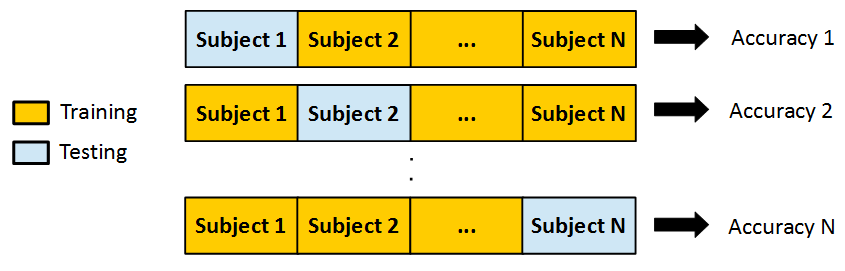
\includegraphics[width=15cm]{Images/LOSOCV.png} 
\caption{ Leave-One-Subjekt-Out-Cross-Validation (LOSOCV): $N$ entspricht der Anzahl der Probanden. Für jeden Split wird ein Testset aus den Daten eines Probanden aufgebaut, während die Daten der anderen Probanden einen Trainingsset bilden. Dieser Vorgang wird für die Daten jedes Probanden durchgeführt. }}
\label{fig:losocv} \end{figure} \vspace{0.5cm}